\newpage
\hypertarget{rules tex}{}
\subsection{Textual TGG Rules}
\texHeader

Rules in the texual syntax are clearly separated into three primary scopes -- source, correspondence, and target -- along with a final scope for constraints,
which can manipulate attributes based on the transformation direction.

\subsection{BoxToDictionaryRule}

\begin{itemize}

\item[$\blacktriangleright$] You may have noticed that a \texttt{Rules} folder was created and included in the TGG package when you first created it. Create
your first TGG rule by right-clicking on this folder and navigating to ``New/TGG Rule.'' Name it \texttt{BoxToDictionaryRule}, and confirm the opened file
in the editor window.

\item[$\blacktriangleright$] Let's first establish the \texttt{source} and \texttt{target} scopes. Given that this is the first rule to be applied in a
transformation, we can assume there is no context to work with, so each of our objects will need to be set to `green' (create). In the \texttt{source} scope,
create a \texttt{box} of type \texttt{Box}. Similarly, in the \texttt{target} scope, create a \texttt{dictionary} of type \texttt{Dictionary}. Your rule
should now resemble Fig.~\ref{eclipse:textSourceRule}.

\vspace{0.5cm}

\begin{figure}[htbp]
\begin{center}
  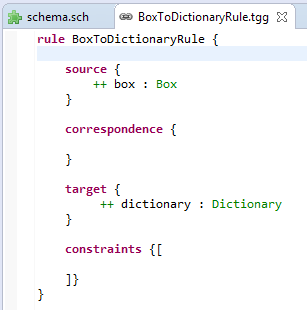
\includegraphics[width=0.5\textwidth]{eclipse_boxToDictionary_start}
  \caption{Creating source and target objects}
  \label{eclipse:textSourceRule}
\end{center}
\end{figure}

\item[$\blacktriangleright$] Now we can create our first TGG correspondence link! In the \texttt{corr\-es\-pond\-ence} scope, enter 

\syntax{++ box <- boxToDictionary : BoxToDictionary -> dictionary}

\item[$\blacktriangleright$] Please note that this statement creates \emph{one} link, named \texttt{box\-To\-Dict\-ion\-ary}, of type
\texttt{Box\-To\-Dict\-ion\-ary} which was declared in the schema.

\end{itemize}

If this rule were to be run at this point, as-is, it would successfully create a single \texttt{Box} and \texttt{Dictionary}! Besides the correspondence link
however, these items have nothing in common. Let's try connecting the \texttt{name} of \texttt{box} to the \texttt{title} of \texttt{dictionary} with an
\emph{attribute constraint}. In TGG rules, attribute constraints provide a bidirectional and high level solution for attribute manipulation. In addition to the
basic math constraints such as addition (add), subtraction (sub), divide, max, multiply, and smallerOrEqual, we have some pre-existing string constraints we can
use. These include stringToNumber, concatenate (concat), addPrefix, addSuffix, and equals (eq).

\begin{itemize}

\item[$\blacktriangleright$] In the \texttt{constraints} scope, write:

\syntax{eq(box.name, dictionary.title)}

Your rule should now resemble Fig.~\ref{eclipse:ruleBasic}.

\vspace{0.5cm}

\begin{figure}[htbp]
\begin{center}
  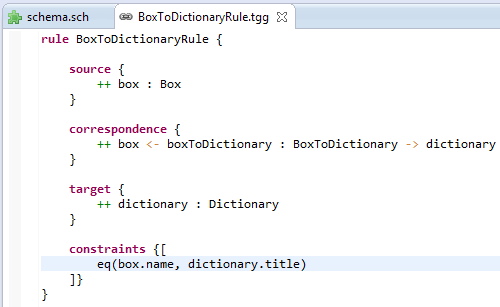
\includegraphics[width=0.8\textwidth]{eclipse_boxToDictionary_firstElements}
  \caption{Creating a correspondence link and adding attribute constraints}
  \label{eclipse:ruleBasic}
\end{center}
\end{figure}

\end{itemize}

We're nearly done, but what's missing from this first rule? We've created the primary container structures for the \texttt{target} and \texttt{source}, and
knowing that entires can be stored directly in \texttt{dictionary}, we know the target scope can remain empty. \texttt{cards} however must be contained within
\texttt{partitions}, so our source scope is till incomplete!

\begin{itemize}

\item[$\blacktriangleright$] Given that there are three difficulty \texttt{level}s for each dictionary \texttt{entry}, create three \texttt{partition}s in the
box that will correspond to the levels: \texttt{partition0}, \texttt{partition1}, and \texttt{partition2}. 

\vspace{0.5cm}

\item[$\blacktriangleright$] Complete the rule by setting both the individual \texttt{index} values and appropriate \texttt{containedPartition},
\texttt{next} and \texttt{previous} link variables so that your rule matches Fig.~\ref{eclipse:allReferences}.

\end{itemize}

\begin{figure}[htbp]
\begin{center}
  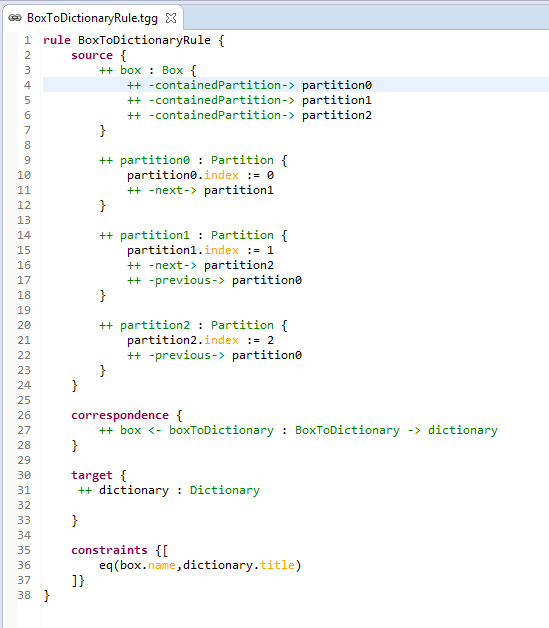
\includegraphics[width=0.8\textwidth]{eclipse_boxToDictionary_complete}
  \caption{The completed \texttt{BoxToDictionaryRule}}
  \label{eclipse:allReferences}
\end{center}
\end{figure}

\clearpage

Great work! This rule is now able to transform a \texttt{box} into a \texttt{dictionary} and vice versa. Unfortunately, it will only be able to handle
completely empty boxes and dictionaries -- you can see we haven't provided any additional handling for \texttt{Card} or \texttt{Entry} items. If you're in a
hurry, feel free to jump ahead to Section 4: TGGs in Action, to try executing this rule anyway. Otherwise, the next rule we create will integrate itself with
\texttt{Box\-To\-Dict\-ion\-ary\-Rule} to take care of this.

% --------------- Card To Entry ------------------------------------------------------------------------------------------------------------------------
\subsection{CardToEntryRule}

\begin{itemize} 

\item[$\blacktriangleright$] Analogously to how you began the previous rule, return to the TGG schema and create a second correspondence type called
\texttt{CardToEntry}, with a \texttt{Card} source and \texttt{Entry} target. Your updated file should now resemble Fig.~\ref{eclipse:updatedSchema}.

\vspace{0.5cm}

\begin{figure}[htbp]
\begin{center}
  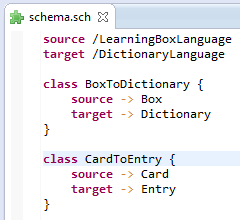
\includegraphics[width=0.4\textwidth]{eclipse_updatedSchema}
  \caption{Updating the schema}
  \label{eclipse:updatedSchema}
\end{center}
\end{figure}

\item[$\blacktriangleright$] Right-click on the \texttt{Rules} folder again, and create the \texttt{CardToEntryRule}.

\end{itemize}

One of the key differences between this rule and the last is that \texttt{Card\-To\-Ent\-ry\-Rule} should only be invoked with a certain context i.e., this will
only be used if a pre-existing \texttt{partition} has \texttt{card} elements that need to be transformed into entries in an established \texttt{dictionary}. In
terms of MOSL, this means there will be both `black' and `green' elements.

\begin{itemize}

\item[$\blacktriangleright$] To begin, create three object variables in the \texttt{source} scope: \texttt{box}, \texttt{partition0}, and \texttt{card}. Which
ones are already known from the context? Which element still needs to be made? Your rule should come to resemble Fig.~\ref{eclipse:c2eRuleSource}.

\begin{figure}[htbp]
\begin{center}
  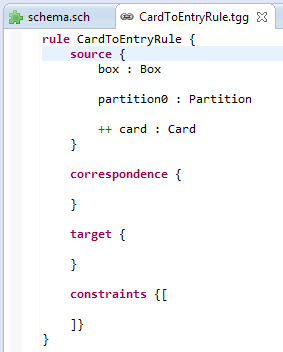
\includegraphics[width=0.45\textwidth]{eclipse_cardToEntry_sourceOVs}
  \caption{The source language with both `black' and `green' elements}
  \label{eclipse:c2eRuleSource}
\end{center}
\end{figure}

\item[$\blacktriangleright$] Similarly, in the \texttt{target} scope, you can demand a `black' \texttt{dic\-tion\-ary:Dic\-tion\-ary} element from the context,
but will need to create a new entry object via \texttt{++ entry:Entry}. 

\vspace{0.5cm}

\item[$\blacktriangleright$] With all of our objects now created, we can complete the \texttt{cor\-res\-pon\-dence}. Our contextual \texttt{box} and
\texttt{dictionary} objects must be connected via the same \texttt{boxToDictionary} link as declared in \texttt{Box\-To\-Dict\-ion\-ary\-Rule}, but a second
link needs to be created between \texttt{card} and \texttt{entry}. Use the correspondence type from the updated schema and write: \syntax{++ card <-
cardToEntry : CardToEntry -> entry}

\vspace{0.5cm}

\item[$\blacktriangleright$] Finally, let's make sure the transformation handles the \texttt{card} and \texttt{entry} attributes correctly. Complete each of
your \texttt{box}, \texttt{partition0}, and \texttt{dictionary} object variable scopes with the relevant references until your rule matches
Fig.~\ref{eclipse:c2eAllReferences}.\footnote{Don't forget that eMoflon's type completion can help you establish references here; Press \texttt{ctrl + space
bar} after writing \texttt{->} for a list of available link variables from the relevant \texttt{eclass}.}

\newpage

\begin{figure}[htb]
\begin{center}
  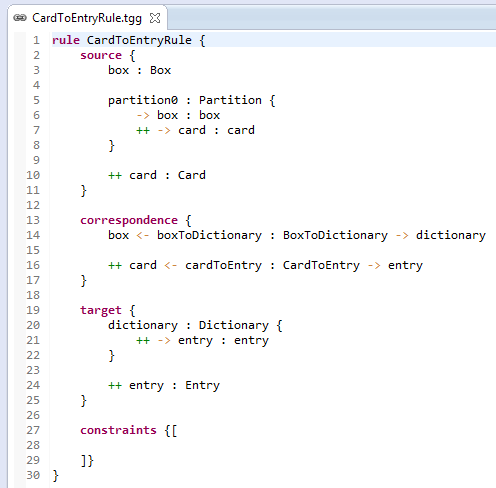
\includegraphics[width=0.8\textwidth]{eclipse_cardToEntry_objectVariables}
  \caption{Rule with all object variables}
  \label{eclipse:c2eAllReferences}
\end{center}
\end{figure}

\end{itemize}

Now let's establish the necessary \texttt{constraints} to handle the relevant content attributes of \texttt{card} and \texttt{entry}. We'll need to
first decide on some common variables and syntax between \texttt{card.face}, \texttt{card.back}, and \texttt{entry.content} so that we can combine each side of
a \texttt{card} into one \texttt{content} value, or split each \texttt{entry} into a question and answer. 

\begin{itemize}

\item[$\blacktriangleright$] Let's define the syntax for \texttt{entry.content} as \texttt{<word>:<mean\-ing>}, \texttt{card\-.back} as
\texttt{Quest\-ion:<word>}, and \texttt{card.face} as \texttt{Answer:<mean\-ing>}. 

\vspace{0.5cm}

\item[$\blacktriangleright$] Using the pre-existing String attribute constraints \texttt{addPrefix} and \texttt{contact} to edit your
\texttt{constraint} scope until it resembles Fig.~\ref{eclipse:contentConstraints}.

\begin{figure}[htbp]
\begin{center}
  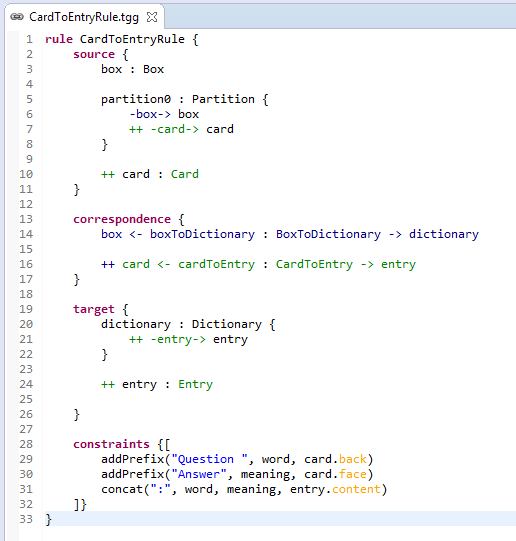
\includegraphics[width=0.8\textwidth]{eclipse_cardToEntry_firstConstraints}
  \caption{\texttt{CardToEntryRule} with its required attribute manipulation}
  \label{eclipse:contentConstraints}
\end{center}
\end{figure}

\end{itemize}

\newpage

We're not quite done -- we need to add \emph{one} more constraint. Given that we have three partitions, and three difficulty levels for each \texttt{Entry}, why
don't we have the transformation assign a level based on whatever partition a \texttt{card} is found in? Hard cards, for example, are more likely to be found in the first
partition (due to being shifted backwards from wrong guesses), while easy cards will be near the end.  As you can imagine, there is no constraint type currently
existing in eMoflon to manage this. We must define our own!

\begin{itemize}

\item[$\blacktriangleright$] Add the following declaration to the \texttt{constraint} scope: \syntax{indexToLevel[BB,BF,FB](EInt, EString)} We will discuss what
each of the options mean in a moment.

\vspace{0.5cm}

\item[$\blacktriangleright$] You can now invoke your rule with an \texttt{indexToLevel(partition0.\-in\-dex, entry.level)} statement immediately below the
declaration. Your completed \texttt{CardToEntryRule} should now resemble Fig.~\ref{eclipse:c2eDone}, where every new \texttt{card} will have an equivalent
(and consistent) \texttt{entry} element.

\begin{figure}[htbp]
\begin{center}
  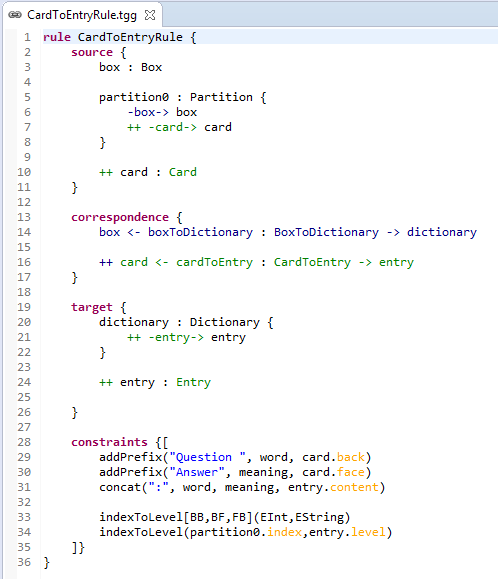
\includegraphics[width=0.9\textwidth]{eclipse_cardToEntry_complete}
  \caption{Completed \texttt{CardToEntryRule} scopes}
  \label{eclipse:c2eDone}
\end{center}
\end{figure}

\vspace{0.5cm}

\item[$\blacktriangleright$] Awesome work! If you haven't already, save the file and confirm the MOSL parser hasn't raised any errors. Press \texttt{Build
(Without Cleaning)} and admire your two TGG transformation rules. 

\vspace{0.5cm}

\item[$\blacktriangleright$] To see how \texttt{BoxToDictionaryRule} is implemented in the visual syntax, check out Fig.~\ref{ea:boxtodictionaryrule_complete}
from Section 4.1. Similarly, \texttt{CardToEntryRule} is depicted in Fig.~\ref{ea:cardtoentry_complete} in Section 4.2.

\end{itemize}
